\documentclass[fleqn, 10pt]{article}

% Paquetes necesarios
\usepackage[utf8]{inputenc}
\usepackage[spanish]{babel}
\usepackage{amsthm}
\usepackage{nccmath} %Para centrar ecuaciones
\usepackage{enumitem}
\usepackage{graphicx}
\usepackage{verbatim}
\usepackage{algpseudocode}




\DeclareMathAlphabet{\pazocal}{OMS}{zplm}{m}{n}
\newcommand{\Lb}{\pazocal{L}}


\theoremstyle{plain}
\newtheorem{proposicion}{Proposición}

\theoremstyle{definition}
\newtheorem{definition}{Definición}[section]
\newtheorem{example}{Ejemplo}[section]

%Definimos el título
\title{Teoría de Autómatas y Lenguajes Formales\\[.4\baselineskip]Práctica 4: Numeración de programas y EXWHILE}
\author{Alba Robles Morales}
\date{27/10/2022}



%Comienzo del documento
\begin{document}

%Generamos el título
\maketitle

\section{Crea el programa WHILE más simple que compute la función de divergencia y computa la codificación de su código }

\begin{algorithmic}
\\X2:=X1+1;
\While{X2!=0 }\\
\\X1:=0;
	
\EndWhile
\\
\\
\begin{center}
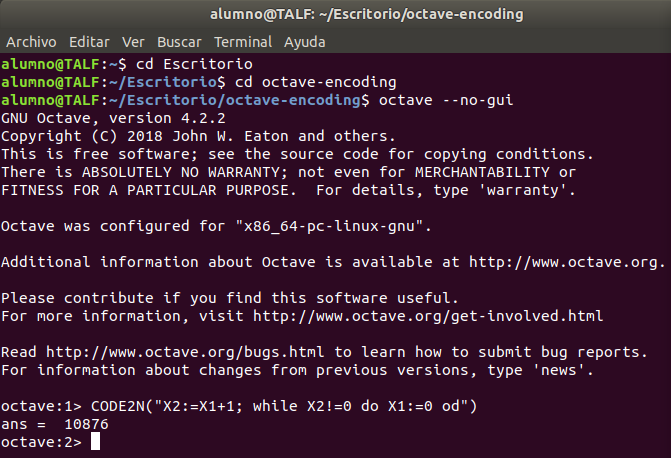
\includegraphics[width=10cm, height=8cm]{pr4_ej1_talf.png}
\end{center}

\end{algorithmic}


\section {Crea un script de Octave que enumere todos los vectores.}
\begin{verbatim}
 
	function printNvectors(5)
for i=0: 4
  disp(['(' num2str(godeldecoding(i)) ')']);
end


function element = godeldecoding(z, k)
## Biyection N -> N*
## godeldecoding(z, k) returns the kth element of the tuple encoded by z
## godeldecoding(z, 0) returns the length of the tuple encoded by z
## godeldecoding(z)    returns the tuple encoded by z
##
## example
##   >> godeldecoding(1258489)
##   ans =
##
##      12    1    7
##   
##  fjv 20180120 GNU GPL v3.0


  ## length of the encoded vector
  if z == 0
    vectorlength = 0;
  else
    vectorlength = cantordecoding(z - 1, 2, 1) + 1;
  end
  ## case to return the length
  if exist('k', 'var') && k == 0
    element = vectorlength;
  else
    ## case to return an element or the vector
    if vectorlength == 0
      ## N^0
      element = [];
    else
      ## N^k, k>0
      ## Cantor number of the vector
      z = cantordecoding(z - 1, 2, 2);
      if exist('k', 'var')
        ## kth element
        element = cantordecoding(z, vectorlength, k);
      else
        ## return the vector
        for idelement = 1:vectorlength
          element(idelement) = cantordecoding(z, vectorlength, idelement);
        end
    end
  end
  
end  


function element = cantordecoding(z, n, k)
## cantordecoding(z, n, k) returns the kth element of the n-tuple encoded by z
## cantordecoding(z, n)    returns the n-tuple encoded by z
##
## example
##   >> cantordecoding(313613413,4)
##   ans =
##   
##      76    8   16    4
##   
##  fjv 20180120 GNU GPL v3.0


  if n == 1
    ## N -> N
    vector = [z];
  elseif n == 2
    ## N^2 -> N
    ## diagonal where the pair is sitting
    diagonal = floor((sqrt(8 * z + 1) - 1) / 2);
    ## the second element is the distance to the beginning of the diagonal
    element2 = z - cantorencoding(diagonal, 0);
    ## diagonal = first element + second element
    vector = [diagonal - element2, element2];
  else
    ## N^k -> N, k > 2
    vector = zeros(1, n);
    for idelement = 1:n - 1
      ## at each level, z encodes a pair of numbers
      pair = cantordecoding(z, 2);
      ## the first element of a pair decodes the elements of the vector
      vector(idelement) = pair(1);
      ## the second element of the pair encodes the rest of the vector
      z = pair(2);
    end
    ## the second element of the pair decodes the last element of the vector
    vector(n) = z;
  end

  if ~exist('k', 'var')
    ## vector as output
    element = vector;
  else
    ## element as output
    element = vector(k);
  end
  
end
  
function code = cantorencoding(varargin)
## Cantor encoding for a vector of numbers of a given length
##
## example
##   >> cantorencoding(3, 3, 3, 3)
##   ans =  82617
##   
##  fjv 20180120 GNU GPL v3.0


  if nargin == 1
    ## case of N
    code = varargin{1};
  elseif nargin == 2
    ## case of N^2
    x = varargin{1};
    y = varargin{2};
    code = (x + y) * (x + y + 1) / 2 + y;
  else
    ## recursive case of N^p, p > 2
    code = cantorencoding(varargin{1}, cantorencoding(varargin{2:end}));
  end
  
end


\end{verbatim}





\section {Crea un script de Octave que enumere todos los programas WHILE.}

\begin{verbatim}
 
	for i=0: 5
  disp(N2WHILE(i));
end


function program = N2WHILE(z)
## Biyection N -> WHILE
##
## example
##   >> N2WHILE(150)
##   ans = (2, while X1!=0 do X1=0 od)
##
##  fjv 20180120 GNU GPL v3.0
##  fjv 20181223 >> transformed from (n,p,s) to (n,s) 


  code = N2CODE(cantordecoding(z, 2, 2));
  
  ## identify the number of each variable
  ## extract the variable in its context (X, followed by digits, followed by : or ; ... or end of string
  [firstchar, lastchar] = regexp(code, 'X\d+(;|=|=!|$)');
  for idvble = 1:numel(firstchar)
    ## extract the number (as a number)
    [~, ~, ~, number]  = regexp(code(firstchar(idvble):lastchar(idvble)), '\d+');
    identifier(idvble) = str2num(number{});
  end
  
  ## extract n
  n = cantordecoding(z, 2, 1);
  ## make while program
  program = cstrcat('(', num2str(n), ', ', code, ')');

end


function element = cantordecoding(z, n, k)
## cantordecoding(z, n, k) returns the kth element of the n-tuple encoded by z
## cantordecoding(z, n)    returns the n-tuple encoded by z
##
## example
##   >> cantordecoding(313613413,4)
##   ans =
##   
##      76    8   16    4
##   
##  fjv 20180120 GNU GPL v3.0


  if n == 1
    ## N -> N
    vector = [z];
  elseif n == 2
    ## N^2 -> N
    ## diagonal where the pair is sitting
    diagonal = floor((sqrt(8 * z + 1) - 1) / 2);
    ## the second element is the distance to the beginning of the diagonal
    element2 = z - cantorencoding(diagonal, 0);
    ## diagonal = first element + second element
    vector = [diagonal - element2, element2];
  else
    ## N^k -> N, k > 2
    vector = zeros(1, n);
    for idelement = 1:n - 1
      ## at each level, z encodes a pair of numbers
      pair = cantordecoding(z, 2);
      ## the first element of a pair decodes the elements of the vector
      vector(idelement) = pair(1);
      ## the second element of the pair encodes the rest of the vector
      z = pair(2);
    end
    ## the second element of the pair decodes the last element of the vector
    vector(n) = z;
  end

  if ~exist('k', 'var')
    ## vector as output
    element = vector;
  else
    ## element as output
    element = vector(k);
  end
  
end



function code = cantorencoding(varargin)
## Cantor encoding for a vector of numbers of a given length
##
## example
##   >> cantorencoding(3, 3, 3, 3)
##   ans =  82617
##   
##  fjv 20180120 GNU GPL v3.0


  if nargin == 1
    ## case of N
    code = varargin{1};
  elseif nargin == 2
    ## case of N^2
    x = varargin{1};
    y = varargin{2};
    code = (x + y) * (x + y + 1) / 2 + y;
  else
    ## recursive case of N^p, p > 2
    code = cantorencoding(varargin{1}, cantorencoding(varargin{2:end}));
  end
  
end
\end{verbatim}





\end{document}